\section*{Zadanie 18.}
\begin{task}
Zdefiniować i zinterpretować (na wybranym przykładzie fizycznym) pojęcie źródłowości pola.\\
\end{task}

\begin{solution}
\textbf{Tutaj nie jestem pewien rozwiązania, bo zwyczajnie nie mogłem odczytać (szczególnie koniec).}\\
Dywergencję dowolnego wektora $\vec{A}$ możemy, na podstawie twierdzenia Gaussa, przedstawić w postaci:
$$\nabla\vec{A}=\lim_{V\to 0}\cfrac{\oiint\vec{A}d\vec{s}}{V}$$
$\oiint\vec{A}d\vec{s}$ - strumień wektora $\vec{A}$ wypływajcego z obszaru o objętości $V$. Dywergencja stanowi stosunek tego strumienia do objętości bardzo malego obszaru. Jeżeli w rozważanym punkcie przestrzeni znajduje się źródł skalarne pola $\vec{A}$ to stosunek ten jest różny od zera i punkt taki nazywany jest polem źródłowym. Jeżeli natomiast dywergencja pola $\vec{A}$ jest równa zero, mówimy o polu bezźródłowym.\\
\begin{center}
$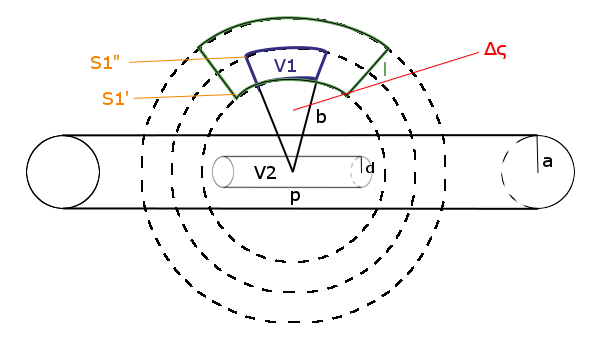
\includegraphics[scale=1]{18_1}$\\
\end{center}
Nieskończenie długi walec o promieniu $a$ naładowany jednoimiennym ładunkiem elektrycznym o gęstości objętościowej $\rho_{V}$.
$$\oiint_{S}\vec{D}\vec{n}ds=\iiint_{V}\rho_{V}dV$$
$$\vec{D}=\vec{i_{\rho}}\cfrac{\rho_{V}\rho}{a},\ \ \rho <a$$
$$\vec{D}=\vec{i_{\rho}}\cfrac{\rho_{V}a^{2}}{2},\ \ \rho >a$$\\ $\rho$ - współrzędne rozważanego punktu w przestrzeni w cylindrycznym układzie współrzędnych.\\
Strumień wektora $\vec{D}$ przepływający przez powierzchnię $S_{1}$ otaczamy obszarem $V_{1}$. Strumień wektora $\vec{D}$ różny od zera przeplywa jedynie przez ścianki $S_{1}^{'} i S_{1}^{''}$. $\vec{D}$ jest równolegly do pozostałych ścianek.
$$\oiint_{S_{1}}\vec{D}d\vec{s}=\oiint_{S{1}^{'}}\vec{D}d\vec{s}+\oiint_{S{1}^{''}}\vec{D}d\vec{s}=
\cfrac{\rho_{V}a^{2}pb\Delta\varphi}{2b} - \cfrac{\rho_{V}a^{2}p(b+l)\Delta\varphi}{2(b+l)}=0$$
Strumień $\vec{D}$ przepływający przez $S_{1}=0$. Pole $\vec{D}$ wytwarzane jest poza obszarem $V_{1}$, przenika przez jego granicę, ale strumień wpływający jest równy strumieniowi wypływającemu. Powoduje to, że pole $\vec{D}$ w $V_{1}$ spełnia $\nabla\vec{D}=0$. Przez mały walec o promieniu $d$, który leży na osi naładowanego cylindra nie przepływa żaden strumień wektora $\vec{D}$, więc możemy rozpatrywać tylko powierzchnię boczną.\\
$\vec{D}$ wypływa z walca przez całą powierzchnię, więc jest zawsze dodatni:
$$\oiint_{S_{2}}\vec{D}d\vec{s}=\cfrac{\rho_{v}d2\pi dp}{2}=\rho_{v}\pi d^{2}p$$
$$\cfrac{\oiint\vec{D}d\vec{s}}{V_{2}}=\cfrac{\rho_{v}\pi d^{2}p}{\pi d^{2}p}=\rho_{v}$$
W obszarze, w którym istnieje niezerowa gęstość objętności ładunków, pole indukcji elektrycznej jest źródłowe, a wartość dywergencji równa się gęstości objętościowej ładunku elektrycznego stanowiącego źródło skalarne tego pola.


\end{solution}